\documentclass[tikz,border=5pt]{standalone}
\usepackage[T1]{fontenc}
\usepackage{lmodern,amsmath,amssymb}
\usetikzlibrary{arrows.meta,calc,positioning,fit,backgrounds,shapes.geometric,matrix,decorations.pathreplacing,patterns}
\definecolor{ink}{gray}{0.08}
\definecolor{wash}{gray}{0.965}
\definecolor{soft}{gray}{0.45}
\tikzset{box/.style={draw=ink,line width=.65pt,fill=white,align=center,inner sep=4pt,outer sep=0pt,font=\small},flow/.style={draw=ink,line width=.65pt,-{Latex[length=1.8mm,width=1.3mm]},rounded corners=2pt},annotation/.style={font=\scriptsize,text=soft,align=center},groupbox/.style={draw=soft,dashed,line width=.45pt,fill=wash}}
\begin{document}
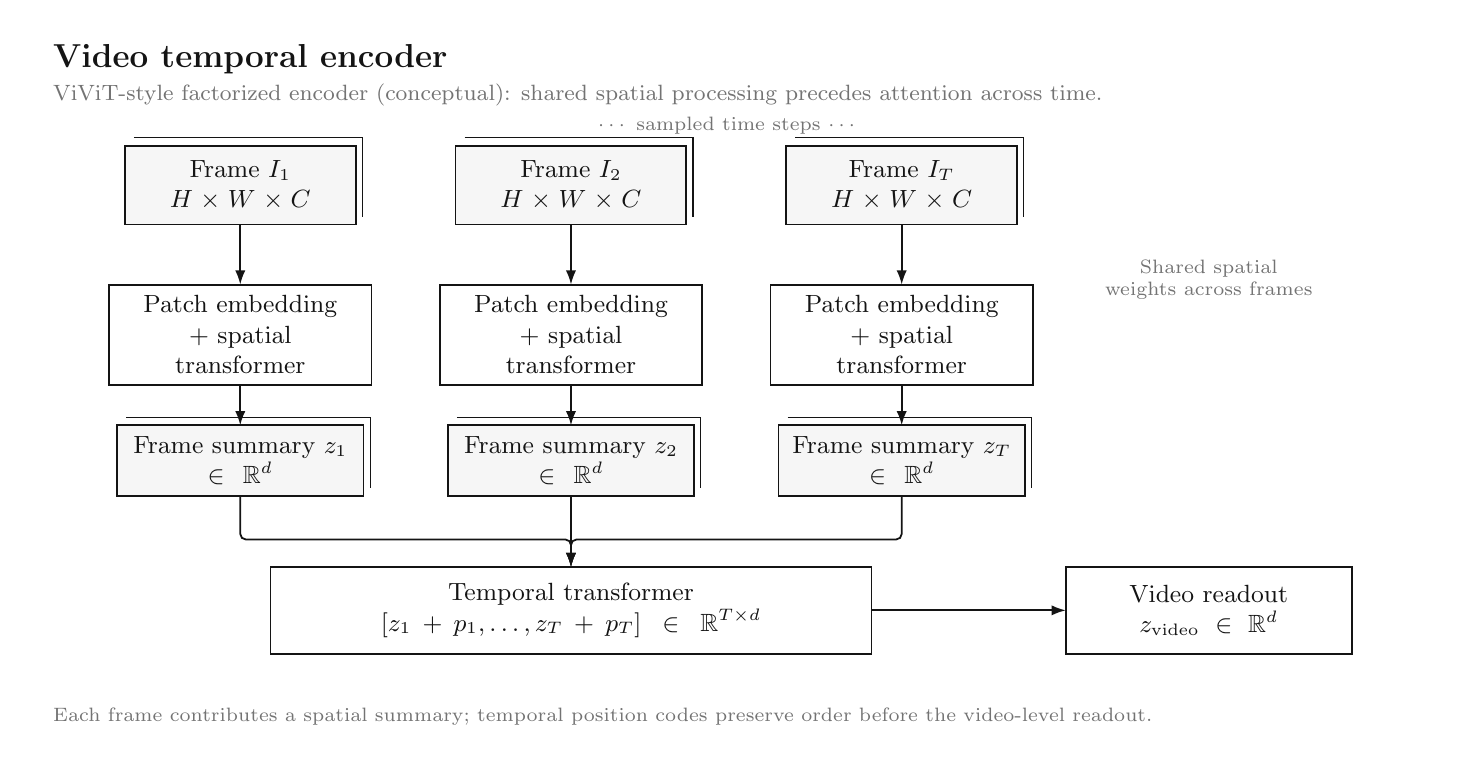
\begin{tikzpicture}[x=1cm,y=-1cm,font=\rmfamily,text=ink]

\path[use as bounding box] (0,0) rectangle (18,9);
\node[anchor=west,font=\large\bfseries] at (.2,.4) {Video temporal encoder};
\node[anchor=west,font=\footnotesize,text=soft] at (.2,.85) {ViViT-style factorized encoder (conceptual): shared spatial processing precedes attention across time.};
\begin{pgfonlayer}{background}
\end{pgfonlayer}
\node[box,fill=wash,minimum width=2.9cm,minimum height=1.0cm,text width=2.65cm] (frame1) at (2.7,2.0) {Frame $I_{1}$\\$H\times W\times C$};
\draw[ink,line width=.4pt] (1.3500000000000003,1.4) -- (4.25,1.4) -- (4.25,2.4);
\node[box,minimum width=3.3cm,minimum height=1.1cm,text width=3.05cm] (spatial1) at (2.7,3.9) {Patch embedding\\+ spatial transformer};
\node[box,fill=wash,minimum width=3.1cm,minimum height=0.9cm,text width=2.85cm] (sum1) at (2.7,5.5) {Frame summary $z_{1}$\\$\in\mathbb{R}^d$};
\draw[ink,line width=.4pt] (1.2500000000000002,4.95) -- (4.35,4.95) -- (4.35,5.8500000000000005);
\node[box,fill=wash,minimum width=2.9cm,minimum height=1.0cm,text width=2.65cm] (frame2) at (6.9,2.0) {Frame $I_{2}$\\$H\times W\times C$};
\draw[ink,line width=.4pt] (5.55,1.4) -- (8.45,1.4) -- (8.45,2.4);
\node[box,minimum width=3.3cm,minimum height=1.1cm,text width=3.05cm] (spatial2) at (6.9,3.9) {Patch embedding\\+ spatial transformer};
\node[box,fill=wash,minimum width=3.1cm,minimum height=0.9cm,text width=2.85cm] (sum2) at (6.9,5.5) {Frame summary $z_{2}$\\$\in\mathbb{R}^d$};
\draw[ink,line width=.4pt] (5.45,4.95) -- (8.55,4.95) -- (8.55,5.8500000000000005);
\node[box,fill=wash,minimum width=2.9cm,minimum height=1.0cm,text width=2.65cm] (frame3) at (11.1,2.0) {Frame $I_{T}$\\$H\times W\times C$};
\draw[ink,line width=.4pt] (9.75,1.4) -- (12.649999999999999,1.4) -- (12.649999999999999,2.4);
\node[box,minimum width=3.3cm,minimum height=1.1cm,text width=3.05cm] (spatial3) at (11.1,3.9) {Patch embedding\\+ spatial transformer};
\node[box,fill=wash,minimum width=3.1cm,minimum height=0.9cm,text width=2.85cm] (sum3) at (11.1,5.5) {Frame summary $z_{T}$\\$\in\mathbb{R}^d$};
\draw[ink,line width=.4pt] (9.649999999999999,4.95) -- (12.75,4.95) -- (12.75,5.8500000000000005);
\node[box,minimum width=7.6cm,minimum height=1.1cm,text width=7.35cm] (temporal) at (6.9,7.4) {Temporal transformer\\$[z_1+p_1,\ldots,z_T+p_T]\in\mathbb{R}^{T\times d}$};
\node[box,minimum width=3.6cm,minimum height=1.1cm,text width=3.35cm] (readout) at (15.0,7.4) {Video readout\\$z_{\mathrm{video}}\in\mathbb{R}^{d}$};
\begin{pgfonlayer}{background}
\draw[flow] (frame1.south) -- (spatial1.north);
\draw[flow] (spatial1.south) -- (sum1.north);
\draw[flow] (frame2.south) -- (spatial2.north);
\draw[flow] (spatial2.south) -- (sum2.north);
\draw[flow] (frame3.south) -- (spatial3.north);
\draw[flow] (spatial3.south) -- (sum3.north);
\draw[flow] (sum1.south) -- (2.7,6.5) -- (6.9,6.5) -- (temporal.north);
\draw[flow] (sum2.south) -- (6.9,6.5) -- (6.9,6.5) -- (temporal.north);
\draw[flow] (sum3.south) -- (11.1,6.5) -- (6.9,6.5) -- (temporal.north);
\draw[flow] (temporal.east) -- (readout.west);
\end{pgfonlayer}
\node[annotation,text width=3.5cm] at (15.0,3.2) {Shared spatial weights across frames};
\node[annotation,text width=5.5cm] at (8.9,1.25) {$\cdots$ sampled time steps $\cdots$};
\node[anchor=west,align=left,font=\scriptsize,text=soft,text width=17.6cm] at (.2,8.75) {Each frame contributes a spatial summary; temporal position codes preserve order before the video-level readout.};
\end{tikzpicture}
\end{document}
